\documentclass{article}
\usepackage[utf8]{inputenc}
\usepackage[letterpaper, margin=1in]{geometry}
\usepackage {graphicx}
\usepackage{amsmath}       % For mathematical typesetting
\usepackage{subfig}         % To create subfigures
\usepackage{subcaption}
\usepackage[modulo]{lineno}    % To make line numbers
\linenumbers                    % To make line numbers
\usepackage{authblk}
\usepackage[table,x11names]{xcolor}   % To allow colors in tables
\usepackage{multirow}           % To make multirows in tables
\usepackage{longtable}          % To make tables spanning more than one page
\usepackage{placeins}
\usepackage[
    backend=biber,
    style=authortitle,
    maxbibnames=99,
    citestyle=authoryear, maxcitenames=2, uniquelist=false,]{biblatex}  % Create the reference  list. 
\addbibresource{landcover.bib}                            % Remember to add the .bib-file in the brackets

\title{Land cover determines threatened and alien species richness in a mixed urban-natural municipality}
\author[1,2,*]{Tanja K. Petersen}
\author[1]{James D. M. Speed}
\author[2]{Vidar Grøtan}
\author[1]{Gunnar Austrheim}
\affil[1]{Department of Natural History, NTNU University Museum, Norwegian University of Science and Technology (NTNU)}
\affil[2]{Centre for Biodiversity Dynamics, Department of Biology, NTNU}
\affil[*]{Corresponding author: Tanja K. Petersen, tanja.k.petersen@ntnu.no}

\date{}

\setcounter{Maxaffil}{0}
\renewcommand\Affilfont{\itshape\small}

\newcommand{\quickwordcount}[1]{%
  \immediate\write18{texcount -1 -sum -merge #1.tex > #1-words.sum }%
  \input{#1-words.sum} words%
}                                                                       % This chunk is to create a simple word-count

\begin{document}
\maketitle

%%TC:ignore
\section{Acknowledgements}
Trondheim Kommune, Marc Daverdin (DTM)

\section{Biosketch}

\newpage
\noindent {\LARGE Land cover determines threatened and alien species richness in an urban-natural municipality}\\  % Title

\textbf{Running title:}   % Make a short running title of less than 40 characters

%TC:break Abstract
\begin{abstract}     
    \textit{Make an abstract here}
\end{abstract}  

\textit{Keywords:} Biodiversity; Land use; Threatened species; Alien species; Urban; Biodiversity management   % Find 6-10 keywords
%%TC:endignore

\section{Introduction}
\subsection{Urbanisation and biodiversity}
% Increasing urbanisation
The majority of the world's population now live in cities, despite these only covering a rather small proportion of the Earth's surface, and urbanisation is predicted to increase (\cite{Grimm2008}, \cite{UnitedNations2018}).
Cities are frequently located in biodiversity hotspots, and  as the increase in urban areas inevitably will happen at the cost of other habitats (\cite{Cincotta2000}, \cite{Araujo2003}, \cite{Kuhn2004}, \cite{Kowarik2011}). In the light of the global anthropogenic biodiversity crisis,  knowledge of the effects of urbanisation and associated factors on biodiversity will be increasingly important with regard to biodiversity management and future urban development (\cite{Pereira2012}, \cite{Johnson2017}). \\ 

% Effects of urbanisation and land cover on biodiversity
Various effects of urbanisation on biodiversity have been suggested and reported, depending on the exact variables in question, and the trends might differ between taxa, such as plants, birds, invertebrates etc. (\cite{McKinney2002}, \cite{Kowarik2011}, \cite{Aronson2014}, \cite{Egerer2017}).
Urbanisation can be a homogenising force, impoverishing the local species pool of native species, while supplying alien species (\cite{Alberti2005}, \cite{Gaston2005}, \cite{Kuhn2006}, \cite{McKinney2002}, \cite{McKinney2006}, \cite{Gaertner2017}, \cite{Padayachee2017}). Thus, alpha diversity might initially seem increased, despite larger-scale beta diversity decrease (\cite{Blair1996}, \cite{Kuhn2006}).\\ 
A review and meta-study by Cadotte et al. (2017) reported that alien species richness generally increases with urbanisation.
In contrast, other studies have linked urban areas with relatively high numbers of native and/or threatened species (see e.g. \cite{Kuhn2006}, \cite{Kowarik2011} and references, and \cite{Ives2016}). Whether this correlation reflects causation, or rather other underlying factors is uncertain. Reasons for an apparent positive correlation between plant species richness and urbanisation can be that the urban habitats frequently offers high habitat heterogeneity with patches of (semi-)natural remnant, allowing species with vastly different requirements to persist (\cite{Francis2015}). Other reasons can be the introduction of alien plant species, e.g. for ornamental purposes, and a natural high productivity independent of human settlement (\cite{McKinney2002}, \cite{Kuhn2004}, \cite{Gaston2005}).\\

% Effects of spatial scale on studies of biodiversity
\subsection{Spatial scale}
These qualitative differences in the effects of urbanisation between studies can also be due to differences in spatial scale of the investigated systems, as the mechanisms underlying species distributions vary with spatial scale (\cite{Borgstrom2006}, \cite{Clergeau2006}, \cite{Pautasso2007}, \cite{Ahrne2009}, \cite{Gerstner2014}, \cite{Concepcion2015}). In some cases large-scale and small-scale variables might interact (\cite{Polce2011}). 
Thus, the chosen spatial resolution is an important factor in analyses of biodiversity (\cite{Deutschewitz2003}, \cite{Gaston2005},\cite{Kuhn2006}, \cite{McKinney2006}, \cite{Ahrne2009}, \cite{Concepcion2016}), and studies have been done on vastly different spatial scales ($>1000\,km$ to meters) (e.g. \cite{Kuhn2006}, \cite{Polce2011},  \cite{Aronson2014}, \cite{Blair1996},  \cite{Gaston2005}, \cite{Ahrne2009}) (\cite{Gaston2000}, \cite{Clergeau2006}, \cite{Pautasso2007}).
However, studies on a fine spatial scale, including a broad urbanisation gradient (ranging from industrialised to natural areas) are largely lacking (but see \cite{Turrini2015a} and \cite{Concepcion2016}).
Pautasso (2007) showed the correlation between human population density (which can be seen as a proxy for urbanisation) and species richness to be highly scale dependent; the correlation being positive on a large spatial scale, but negative on a small spatial scale (threshold: spatial grain of approx. $1\,km$).
Thus, in the case of local biodiversity management, a relatively fine spatial scale is likely necessary to capture potentially negative correlations between human settlements, more detailed land cover variables and species richness, rather than the more general global biogeographic effects (\cite{Gaston2005}).  
Similarly, if the results of biodiversity research is to be used by local management, it is crucial that these results are obtained and delivered on a scale and with an extent appropriate for potential management intervention.\\

% Multi-species vs. single-species approach, and focus on threatened vs. alien species
\subsection{Narrow vs. broad taxonomic framework}
Studies on species distributions and diversity are often done for single species or for  restricted taxonomic groups (e.g. \cite{Kattwinkel2009}, \cite{Milanovich2012}, \cite{Turrini2015a}, \cite{Ives2016}, \cite{Egerer2017}). % more examples here, as I find them!
However, most direct biodiversity management is done on a local- rather than national scale, and public management will seldom be involved in management of single species. Instead, patterns across multiple taxonomic groups are of interest.
High resolution data on single species are limited (\cite{Guisan2000}). Including multiple taxa (and thus generalising the predictors) could increase the amount of available data considerably, thus giving a larger sample size (\cite{Stockwell2002}, \cite{Graham2004}). \\
Modelling a high number of species simultaneously will decrease the potential for for detailed modelling, as we are unlikely to find variables important across multiple taxa (\cite{Chapman2011}). 
However, if more general statements regarding overall biodiversity are needed, as is likely the case for local management, models with such detailed variables are potentially unnecessary. Rather, generalised remarks, based on less detailed variables can be incorporated into biodiversity management. Land use variables have been shown to influence measures of species richness, and thus serve as potential candidates for such overarching factors (\cite{Gerstner2014}). Guisan et al. (2000) suggests that when modelling distributions on a small scale, indirect parameters, such as land cover, will provide the best predictions.\\ % (more sources?)
For conservation purposes, not only overall biodiversity is of interest. Native, threatened species  and alien species are frequently in focus (e.g. in the Norwegian `Natural diversity' law (\cite{nml2009})). 
Especially the similarities and differences in variables determining their distributions, respectively.  Knowledge of how broad land cover variables affect the distribution and richness of these groups could help guide decisions on city development and biodiversity management on municipality level.\\ % sources?

% Data availability and choice of variables --> management
\subsection{Data availability}
Large amounts of data on species distributions can now be retrieved from data available from online databases, such as the Global Biodiversity Information Facility (GBIF) (\cite{GBIF}). \\ 
The use of such databases can be beneficial, as they can provide large data-sets without great costs, and without the need for intensive manual labour, e.g. through the sampling and mapping of species (\cite{Graham2004}).\\
Modelling species richness and distributions frequently require very specific and detailed environmental information. Retrieving data on these variables can be quite laborious, and they might not be feasible to retrieve on a sufficiently fine spatial scale  (\cite{Guisan2000}). 
Similarly, data on highly species specific variables, or ones which require substantial work to obtain, might be of little use to management. In such a context, there is a need for using easily obtainable data, and preferable data used by other branches of public management, to ease cooperation and transfer between departments.\\
%With regards to management and conservation of biodiversity, it is desirable to have overarching models of species richness to ease decision making, and the construction of such models should preferably be quite general, and use easily obtainable data, such as land cover.  Such models would provide useful, general guidelines for future management and city development.\\  % Elaborate and add some sources   % This chunk might not be relevant anyways

% Predictions/hypotheses
Trondheim municipality is fairly well-sampled with regards to occurrence records in GBIF, among other things due to the presence and activity of the University Museum.
Detailed maps of land cover and land use are continuously made by the municipality, and these are used by multiple management organs. The land cover data is locally produced and updated by the municipality, but collected and distributed centrally, ensuring a streamlined classification system across all of Norway (\cite{SOSI}). 
As multiple management decisions are made on a municipality scale in Norway, using the municipality as the spatial extent of biological investigations is sensible.\\ % Elaborate? I am not quite certain if this paragraph should be kept, or if it is presented sufficiently in the Method-section

\subsection{Aim and hypotheses}    
The aim of this study is to investigate which general, fine-scale land cover variables influence the threatened and alien species richness in a northern European  municipality, covering a broad urbanisation gradient. We hypothesise the following:\\
\textbf{Urban areas} are positively associated with alien species, as cities are thought to function as introduction sites for (plant) species associated with gardens. Similarly, key pathways for introduction of alien species are through trade and alike, which are more prevalent in urban areas than outside (\cite{Pysek1998},\cite{McKinney2002}, \cite{Deutschewitz2003}, \cite{Kuhn2006}, \cite{McKinney2006}, \cite{Kowarik2011},\cite{Polce2011}, \cite{Genovesi2013},\cite{Cadotte2017}, \cite{Padayachee2017}). 
The association with threatened species might be either positive due to natural high species richness, or as the highly disturbed nature of urban areas might provide small suitable habitat patches for specialised species, or negative due to the vast amount of disturbances (\cite{McKinney2002}, \cite{Kuhn2004}, \cite{Kowarik2011}, \cite{Aronson2014}, \cite{Ives2016}).\\
\textbf{Forests} are likely to be positively associated with both threatened and alien species, as approx. 48\% of the Norwegian Red-listed species are generally associated with forests, and that several alien tree species have been planted for forestry (\cite{Presto2005}, \cite{Presto2013}, \cite{Henriksen2015}). The associations might depend on more fine scale forest composition and structure (out of the scope of this study).\\
\textbf{Open areas with sparse vegetation} (or otherwise disturbed habitat) are associated with alien species, as these are frequently hypothesised to be pioneer species or in other ways capable of exploiting disturbed habitat (\cite{Maskell2006}, \cite{Kowarik2011}, \cite{Polce2011}, \cite{Cadotte2017}).\\
\textbf{Areas including ecotones} will harbour a high number of species, as these generally provide contrasting habitat types and frequent disturbances, catering to different species (\cite{Lloyd2000} and references, \cite{Walker2003}, \cite{Maskell2006}). In this study, this should be especially true for edge zones between land and sea, and land and limnic areas.  \\
\textbf{Habitat heterogeneity} affect both groups positively, as more diverse habitat within an area provide resources for different species (\cite{Araujo2003}, \cite{Deutschewitz2003}, \cite{Sattler2010}, \cite{Aronson2017}, \cite{Matthies2017}).\\
\textbf{Topography} can influence species richness, as especially plant species are negatively associated with north-facing slopes, due to a lack of light (\cite{Holland1975}). Thus, north-facing slopes are expected to be negatively correlated with overall species richness.


\section{Materials and methods}
All analyses were performed in R, version 3.4.4 (\cite{R}).\\

\subsection{Study area}
The study was done within the Trondheim Municipality (Norway) administrative borders. Trondheim is located around $63.42\,^{\circ}N$,  $10.38\,^{\circ}E$, and is a temperate, coastal municipality with an area of $342\, km^2$, a population of approximately 190,000 people (\cite{TrondheimKommune2018}), and annual mean temperature and precipitation is approx. $5\,^{\circ}\mathrm{C}$ and $887\, mm$ (\cite{ssb2018}).\\
Within the municipality border exists a full urbanisation gradient; from city centre and industrial areas to natural areas, managed to favour biodiversity. The municipality covers highly different nature types, including both coastline, mountainous areas and limnic systems, thus having a large potential for varied biological communities and high levels of biodiversity (\cite{TrondheimKommune2018}).\\
% Write something about the urban-rural gradient

\subsection{Data retrieval and data cleaning}
\subsubsection{GBIF occurrence records}
All occurrence records from within a polygon around the Trondheim Municipality administrative border were downloaded from Global Biodiversity Information Facility (GBIF) (GBIF.org (March $6^th$ 2018) GBIF Occurrence Download  https://doi.org/10.15468/dl.ruacxc). The initially used polygon was created to ease the download; the data was filtered according to the administrative border in subsequent steps. The data-set was then filtered to only including data matching the following criteria:
\begin{enumerate}
    \item Records should contain a full species name (no occurrence records identified only to higher taxonomic levels), to ensure validity of the finding, and to make it comparable to the used lists of threatened and alien species.
    \item Records should have a coordinate uncertainty of $\leq354 \,m$. This was done to match the spatial resolution of the analyses. The $354\, m$ equals half the length of the diagonal of the $500\, m \times 500\, m$ grid cells, thus specifying the maximum distance from the centre coordinates still within the grid cell.
    \item Records should have coordinates falling within the Trondheim Municipality administrative border. %insert source of shapefile
    \item Records should have been recorded after (and including) year 2013 to ensure compatibility with the used land cover maps.
\end{enumerate}

The resulting data-set was further divided into two subcategories: threatened species and alien species.\\
The species included as `threatened' were defined based on one or more assessments of the national Norwegian Red List from 2006, 2010 and 2015, provided by The Norwegian Biodiversity Information Centre. The species on these lists are the ones categorized (locally) within the official IUCN categories `Data Deficient' (\textit{DD}),  `Near Threatened' (\textit{NT}), `Vulnerable' (\textit{VU}), `Endangered' (\textit{EN}), `Critically Endangered' (\textit{CR}), `Regionally Extinct' (\textit{RE}). See Supplementary material (section \ref{sec:Redlist_criteria}) for detailed description of inclusion details.\\
The species defined as `alien' were defined based on the Alien Species List (2012) from The Norwegian Biodiversity Information Centre. Only species alien to mainland Norway were retained (excluding species only alien to Svalbard). Thus, all alien species were are included, regardless of risk category. This was opted for due to a lack of data otherwise.\\
Nomenclature were resolved using the Taxonomic Name Resolver (function \textit{"tnrs"} from the \textit{taxise}-package); as the names used in the Norwegian Red List and the Alien Species List occasionally do not match the names used in GBIF, potential synonyms were identified. When filtering the full data-set into subsets, both the names from the official lists and accepted synonyms were used.\\
Only terrestrial and limnic species were included in the data-sets. All species classified as marine by The Norwegian Biodiversity Information Centre were manually excluded from the lists (excluding birds, as all bird species in the data-set were regarded as somewhat terrestrial).\\

As the data used in this study are downloads from an online database (GBIF), the records are of fluctuating quality. By far, the most records are ``human observations'', and the most records are provided by the Norwegian Ornithological Society. As a large part of the data-set is likely unvalidated sightings, there is no guarantee that the data-set is without errors. However, it is assumed that by cleaning the data as described above, the number of potential mis-identifications is diminished. Likewise, as the individual species are not analysed, it is unlikely that single erroneous records will highly affect the aggregated species pool.\\
There is a risk that some records of alien (plant) species can be recordings from inside private gardens. However, as by far the most the records of plants are reported by skilled amateurs and professionals (institution: Norwegian Botanical Society), and by scientific institutions (NTNU University Museum herbarium), it is assumed that the influence of these potential errors are negligible.\\

\subsubsection{Land cover data}
Land cover was based on the Norwegian AR5 maps (Land Resource map 1:5000) from the \cite{AR5}. 
Shape-files of the land cover maps were provided by the Trondheim Municipality in April 2018. The AR5 maps are both continually and periodically updated, and provides the most complete data on national land resources. % source: https://www.nibio.no/tema/jord/arealressurser/arealressurskart-ar5/.
Land resources are categorised based on land cover type, tree cover (coniferous, deciduous or mixed trees), timber productivity and soil condition, giving 106 potential AR5-categories. Of these, 66 functionally unique categories are present within Trondheim municipality (hereafter called ``land cover types'') (see Supplementary Material, section \ref{sec:Landcover_clusters}, Table \ref{table:AR5_classes}).
The map was overlaid by a grid ($500\,m \times 500\,m$), and the areas of each land cover type present in each grid cell were calculated.\\

Aspect slope of the terrain was included as a potential land cover variable.  The data on aspect was taken from a Digital Terrain Model raster with a solution of $25\,m \times 25\,m$. The circular aspect (unit: degrees) was transformed to a "Northness"-measure by
\begin{equation*}
\text{Northness} =\text{cosine}(\text{Aspect slope}\,(^\circ)),
\end{equation*}
hence fitting a scale of $(-1)$ to $1$ (in this definition: $(-1)$ = south-facing, $1$ = north-facing). All flat areas were given $NA$-values. For each grid cell, "Northness" was calculated as the mean of all raster cell within the overlaid grid cell. 

\subsection{Preparation of variables}
\subsubsection{Extrapolated Species Richness (ESR)} \label{sec:data_criteria}
All of the retained GBIF records were assigned to the corresponding grid cell. For each grid cell, the number of records and the number of individually observed species were calculated. Due to differences in sampling effort across the study area, the number of observed species within each grid cell was deemed an unreliable measure. To deal with the issue of differential exposure, the Extrapolated Species Richness rather than observed species richness was used.
 A community matrix was constructed ($\text{Grid cell number} \times \text{Species name}$), and the Extrapolated Species Richness (ESR) for each grid cell calculated, using the \textit{"estimateR"}-function from the \textit{vegan}-package. This function uses an equation similar to the bias-corrected Chao's method:
    \begin{equation*}
        S_p = S_0 + \frac{a_1 (a_1-1)}{2(a_2 + 1)} ,
    \end{equation*}
where $S_p$ denotes the estimated species pool, $S_0$ denotes an estimate of number of unseen species, $a_i$ denotes the number of species with $i$ individuals (\cite{Oksanen2017}). % Remember to reference the vignette! https://cran.r-project.org/web/packages/vegan/vignettes/diversity-vegan.pdf
    
For each of these estimates, the variance of the estimate was calculated as well, which in turn was used to calculate the standard error of the estimates.
These calculations were done for all species, threatened- and alien species individually.\\

As some of the estimates from this extrapolation are rather uncertain, some "pruning" of the grid cells was necessary. Similar to the methods described in Ballesteros-Meija et al. (2013), only grid cells having a minimum number of records ($\geq10$) and a maximum coefficient of variation ($\leq0.25$) of the total ESR were included in the further analyses. The coefficient of variation was calculated as $ \frac{\text{Standard error of ESR}}{\text{ESR}}$.

\subsubsection{Land cover variables}
The 66 different recognised land cover types were too many to fit in a model given the available data, and the number had to be reduced. As subjectively selecting land cover variables opposed the aim of determining the influential variables, hierarchical cluster analysis was used to identify grid cells with similar composition, thus creating a limited number of clustered land cover type categories.\\
All grid cells within the administrative border of the Trondheim municipality were used for the cluster analysis, including cells only partially within the municipality border; in that case, only the within-municipality area was used. Grid cells only covered by ocean were not included ($\text{area of ocean} = \text{total area}$). The cluster analysis was done using the function \textit{``hclust''} on a dissimilarity matrix based on the AR5 land cover in each grid cell. \textit{``Complete linkage''} was used as the clustering method. The dissimilarity matrix was made with the function \textit{``vegdist''} from the \textit{vegan}-package, based on the Bray-Curtis dissimilarity between the individual grid cells.\\
The optimal number of clusters for the given dissimilarity matrix and clustering method was determined to be $11$, based on the \textit{``Nbclust''}-function, comparing multiple indices of optimal cluster value. The corresponding dissimilarity cut-off value lead to some clusters containing very few grid cells ($\leq{3}$). which was evaluated to be too few for meaningful analyses. Thus, the cut-off value was set at $0.99$, resulting 11 clusters containing $> 3$ grid cells.
Each cluster will hereafter be referred to as a ``habitat''.\\

The Simpson's Diversity Index was calculated for each grid cell to take into account habitat heterogeneity within each grid cell. The index is calculated as $1-D$, where $D$ is:
\begin{equation*}
    D = \sum (\frac{n}{N})^2 ,
\end{equation*}where $n$ is the total area of a particular land cover types, $N$ is the total area of the grid cell. The index ranges between $0$ (completely homogeneous land cover) and $1$ (infinite heterogeneity in land cover).\\
Number of land cover types ($S$) and the evenness of land cover types ($\frac{1}{D}/S$) within in each grid cell were considered as potential variables, but both proved to be colinear with habitat heterogeneity, and were thus not included in the models.\\

\subsection{Modelling ESR based on land cover variables}
The response variables ($ESR_{all}$, $ESR_{threatened}$ and $ESR_{alien}$) were log-transformed ($log(x+1$)) to ensure normality. One grid cell including a suspiciously high number of alien species was removed from the analysis as an outlier. The grid cell included the Ringve Botanical garden, and the number of reported alien species here is thus unlikely to be representative of the environmental conditions, and three additional grid cells were removed due to missing data. These included only completely flat areas ($northness=NaN$) and were fully covered by freshwater.\\
    
Two linear models were created for each of the three species groups (all, threatened and alien): one modelling the log-transformed Extrapolated Species Richness, and one in which the response variable was scaled and centered to allow for comparison of variable effect sizes across models. Centering is done by subtracting the mean value from from the corresponding value, scaling is done by dividing the (centered) values by the standard deviation of the mean (function "\textit{scale}").\\
Due to spatial autocorrelation in both data and preliminary model residuals ($\text{Moran's I}>1$ within the defined neighbouring distance of $1.5 km$ for all three species group models, function \textit{"moran.mc"} in the \textit{spdep}-package, 999 permutations), models were formulated as patially explicit generalised least squared (GLS) models (exponential correlation structure, package \textit{nlme}). The models were fitted using Maximum Likelihood:
        \begin{equation*}
            log(ESR + 1) = Habitat + Habitat\, heterogeneity + Northness,
        \end{equation*}

To identify the best model, a number of candidate models were evaluated (the model described above indicating the most extensive model, other models being subsets of this) and compared by $AIC_c$, using the functions \textit{``dredge''} and \textit{``model.avg''} from the \textit{MuMIn}-package. The best-ranking models ($\Delta AIC_c < 2 $, as suggested by Burnham and Anderson (2004) were used for a weighted average model (\cite{Burnham2004}).\\ 
Models with both the original and scaled response variable, $log(ESR+1)$, were constructed. A $\text{pesudo-R}^2$ was calculated as the correlation between the predicted values versus the observed values (\cite{Ballesterosmejia2013}). 
The models were used to predict the ESR estimates across all grid cells within the Trondheim municipality.\\

\section{Results}
\subsection{Available data}
The number of records downloaded from GBIF was $864,715$ ($9,117$ unique species names, $48,468$ records not identified to species level). 
When the data was cleaned according to the mentioned criteria, the number of records was reduced to $251,803$ ($3,097$ unique species names). Of these, $32,585$ (121 unique species names) could be categorised as threatened, and $3,447$ (177 unique species names) as alien. \\
The total number of grid cells within Trondheim municipality not entirely covered by ocean is 1509. After applying the "pruning" criteria, these were reduced to 295. Removing the outlying grid cells and the grid cell with missing Northness-data, the final number is 291.

\subsection{Land cover variables}
The cluster analysis identified 17 habitats at the chosen cut-off. Of these, 6 included $\leq3$ grid cells. These were mainly found on the municipality border, thus being cells with a significantly smaller area than the majority of the grid cells. These were excluded from further analysis.\\
The mean area of each land cover type within the clustered cells were calculated, and the habitats were named according to the (on average) dominating land cover types within the cells. A map coloured by habitats can be seen in Figure \ref{fig:Clusters}. A spineplot identifying the land cover characteristic of the habitats can be seen in the Supplementary material (fig. \ref{fig:spineplot}, Section  \ref{sec:Landcover_clusters}).\\
The number of grid cells classified as each habitat can be seen in Table \ref{\ref{table:AR5_classes}}. The most frequent habitat within the municipality was Cultivated land, followed by Coniferous forest and Urban/developed areas. This distribution was not seen in the grid cells included in the model construction; here the most frequent habitat was by far Urban/developed areas, followed by Cultivated. This illustrates the strong bias in sampling effort.\\
\textit{`Open firm ground and forest'} (Habitat 10) could not be included as a factor level in the modelling, as no grid cells from this habitat had enough data, according to the criteria listed in the methods (section \ref{sec:data_criteria}), to be included in the models.\\

\subsection{Modelling and model predictions of ESR}
The summary of the model comparisons can be seen in the Supplementary Material (Table \ref{table:model.sel} and Table \ref{table:model.sel.std}, Section \ref{sec:model_sel}).
For the threatened species, only one model was evaluated `best-ranking', according to the described criteria, whereas two candidate models were averaged for both all species and alien species. In all cases, the final models were of the form
$gls(log(ESR + 1) \sim \text{Habitat} + \text{Habitat heterogeneity} )$. \\
For the total species richness, both candidate models included habitat heterogeneity, whereas only the second highest ranking model included both predictors. For the alien species, both candidate models included Habitat, but only the highest ranking model included both predictors.\\
Model coefficients are shown in Table \ref{table:model_parameters}, \ref{table:model_parameters.std} and Figure \ref{fig:pred_ribbon} in the Supplementary Material, section \ref{sec:models}, and are visualised in Figure \ref{fig:coefficients}. For the averaged models, the full model average rather than the conditional average was used, to better determine which predictors had the strongest effects on the ESR (\cite{Grueber2011}).\\
The largest effect sizes for total species richness originate from `Coastal' habitat - however, there are no significant differences in the effect sizes of the different habitats in the full model average, due to the decreased weighting of this variable. Significant differences could potentially have been seen in the conditional model averages.
Threatened species richness is mainly affected by `Coastal' habitat. The effect sizes of the different habitat levels were not all significantly different. 
The largest effect sizes for alien species richness is from the Habitats `Coastal', `Urban/developed' and `Urban/vegetated/riparian'. Similarly, not all habitat levels were significantly different.\\
The $\text{pseudo-R}^2$ for the models indicates that the best model fit is achieved for the threatened species ($\text{pseudo-R}^2= 0.594$), followed by the alien species ($\text{Pseudo-R}^2= 0.473$) and lastly all species ($\text{Pseudo-R}^2= 0.304$) (Table \ref{table:model_parameters} and \ref{table:model_parameters.std}).\\
The model predictions are shown in Figure \ref{fig:ESR_predictions}. The visualised numbers have been back-transformed to represent actual species numbers. The predicted total number of species ranged from $27.5$ to $101.8$ species ($\text{mean = } 61.81$ and $\text{median = }61.3$), threatened species ranges from $-0.16$ to $15.7$ species ($\text{mean = } 3.33$ and $\text{median = } 3.26$), and alien species ranged from $-0.04$ to $2.9$ species ($\text{mean = } 1.0$ and $\text{median = } 1.0$) pr. grid cell.

\section{Discussion}
% "Mini abstract" - ease the reader into the discussion
We used GBIF records and official land cover classifications to determine how habitat affects total species richness, and number of threatened and alien species. We did so by constructing GLS models based on habitat, habitat heterogeneity and mean aspect within $500 m \times 500 m$ grid cells across the Trondheim municipality, selecting the best candidate models based on $\Delta AIC_c$ and model averaging. The best, averaged models in all cases predicted Extrapolated Species Richness as a function of habitat and habitat heterogeneity. The highest predicted number of threatened species were in coastal areas, and areas with high levels of habitat heterogeneity. The highest predicted number of alien species were in coastal, urban and developed areas. Habitat heterogeneity was a less influential predictor for alien species richness than for total or threatened species richness. 

\subsection{Model performance}
Of the total 1509 grid cells (excluding cells fully covered by ocean), only 291 were adequately sampled to allow for analyses. These are heavily biased towards urban areas, supporting the general trend in citizen science data, of being biased towards inhabited or areas otherwise accessible to the public (\cite{Graham2004}). % Insert sources!
Especially areas within Trondheim municipality relatively far from human activity are under-sampled, with one habitat not being represented in the analyses at all. Unfortunately, this leaves the habitat ``Open firm ground'' relatively unexplored.\\ %Similarly, no habitats characterised by grasslands were identified, leaving this hypothesis untested. \\
For all three species groups, the best models predicted ESR as a function of habitat and habitat heterogeneity. Threatened species was the only group for which only a single candidate model ranked best. For both other species groups, two candidate models could not be differentiated, and they were averaged to give the final models. The two highest-ranking models describing alien species richness both included habitat, but only one included habitat heterogeneity. Of the highest ranking models describing total species richness, habitat heterogeneity was included in both, whereas habitat was only included in one. \\
The relatively poor fit of the models and the observed values ($\text{Pseudo-R}^2$ ranging between $0.304$ and $0.594$) can likely be ascribed to several factors. One being that the ESR itself is surrounded by quite some uncertainty, as it is already an extrapolation. Whether the ESR is a valid proxy for species richness is debatable. As the models are purposefully rather crude, they are inevitably lacking important predictor variables, which would likely have increased the explained variance. However, including highly detailed variables was not the the aim of this study. As the data-set included a wide array of species, these are bound to not respond in similar ways to variation in the included variables, or to the important variables not included. As the study did not include information on the identity of the individual species, these effects cannot be directly identified.   % Add some sources here regarding some of the uncertainties

\subsection{Effects of land cover variables}
When comparing the model coefficients (both scaled and unscaled) of the three models (Figure \ref{fig:coefficients}.a, Figure \ref{fig:coefficients}.b, Table \ref{table:model_parameters.std}), it is evident that the various habitats have a significantly different effect on the three species groups.\\
% Habitats
% Coastal areas
Coastal areas are seemingly the habitat with the highest number of threatened species, though the scaled effect size is comparable to that of the alien species. The influence of this variable on total species richness is less than for the two subgroups.
The high number of both threatened and alien species in coastal habitats can likely be ascribed to these habitats being ecotones, proving highly contrasting habitats. Ecotonal species are often exotic species (\cite{Walker2003}), and ecotones have generally been suggested to have an increased species richness compared to other habitats. In contrast, Lloyd et al. (2000) found ecotonal species to mainly be natives, which is supported by the findings here, when considering the differences in species numbers.\\
% Urban
The scaled effects of urban areas on species richness are comparable for total and threatened species, but alongside coastal areas, the two urban habitats are the ones with the most alien species, and the scaled effect size is significantly higher than for the other species groups.
The association between alien species and urban areas is not surprising, as cities act as introduction sites and centres of spread, mainly due trade and traffic (\cite{Pysek1998}, \cite{Francis2015}, \cite{Padayachee2017}).
This is similar to the findings of Deutschewitz et al. (2003), who found both native and alien plants to be positively influenced by urban areas, but the effect size being larger for alien plant species than for the native ones. Similarly, the review by Kowarik (2011) found cities to be hotspots of alien plant species.\\
The apparent link between urban areas and species richness is not necessarily a stand-in for the presence of self-sustaining populations. It is possible that the urban areas are functioning as `ecological traps', and the populations or individuals found herein have an extinction debt to pay (\cite{Blair1996}, \cite{McKinney2002}, \cite{Kowarik2011}). Urban areas can potentially favour a few, urban adapted species, leading to a high abundance of these, but potentially decrease species evenness (thus making the community dominated by a few urban exploiters, despite housing a large number of species) (\cite{Turrini2015a}).\\
Urban land cover have previously been shown to negatively affect species richness of birds and plants, whereas species richness is positively associated with the cover of intact vegetation within an urban setting (\cite{Aronson2014}). However, as the predictors in this and the referenced study are vastly different, the results are not necessarily in opposition to one another. The positive effect of vegetation cover within the urban setting, is potentially captured within the habitat heterogeneity variable presented here.\\
% Forest
Contrary to expectations, the effect size of the various forest habitats on threatened species is lower than for most other habitats, and for two out of three forest habitats, it is significantly lower than for the other species groups.
The lack of threatened species in the forested areas can be due to the lack of sampling, thus showing a spatial bias in the data rather than a biological skew. However, large parts of the forested areas in Trondheim are largely affected by previous afforestation for timber production, in which mainly coniferous species (both native and alien) were planted (\cite{Presto2005}). These forests might not provide the needed resources for native species (\cite{Brockerhoff2008}).
% Habitat heterogeneity
As expected, habitat heterogeneity has a positive effect on species richness, both for the total number, and for the threatened and alien species. The effect on alien species is significantly smaller than for the other species groups, however. This, to some extent, supports the results of Matthies et al. (2017) and the meta-analysis by Beninde et al. (2015), in which respectively habitat heterogeneity and habitat richness was positively associated with species richness in urban areas.
This positive correlation between habitat heterogeneity  and species richness have been observed in multiple studies of more restricted taxonomic groups (\cite{Sattler2010}), (\cite{Deutschewitz2003}, \cite{Matthies2017}).   %find more references!
Habitat heterogeneity likely allows for multiple smaller niche pockets, thus allowing a diverse array of species having their requirements fulfilled (\cite{Tews2004}).\\ % Discuss this a little more, maybe?
Aspect slope was not a significant variable in this study. This likely relates to the potentially differing associations with topography between taxonomic groups, and the spatial scale of the study; topography likely influences organisms on a much smaller scale than the one used here.\\
 
 As the variables used in these models are ``indirect'' (\textit{sensu} \cite{Guisan2000}), they is no mechanistic underpinning of the correlations with species richness; the habitats rather function as proxies for other parameters. For that reason, a direct extrapolation for other geographical areas should be cautious (\cite{Guisan2000}). However, the methods are highly applicable in other areas.
   
\subsection{Data uncertainty}
As seen in other studies, % find some sources, potentially
the data was spatially biased towards inhabited areas (\cite{Graham2004}). This unfortunately means that large areas with minimal human influence are heavily under sampled, potentially skewing the results. Attempts to take this sampling bias int account was made; however, large areas are still left uninvestigated. The sample sizes (number of records within each species group) were quite different, with many more observations of threatened than alien species. Whether this indicates and actual difference in numbers, or a reporter bias is uncertain. Aronson et al. (2014) found cities across the globe to contain more native (though not necessarily threatened) bird and plant species than alien ones, thus supporting the results shown here.
However, as large parts of the data-set originate in citizen science, wherein there might be a greater incentive to report threatened or otherwise rare species compared to either common or alien species.\\ % find some sources

\subsubsection{Taxonomic bias}
The data from GBIF is strongly taxonomically biased, with most of the downloaded records being birds. In all subsets of the data, birds are vastly over-represented, but more so among the threatened species and in the overall data-set. This is likely due to the high activity of amateur ornithologists among community scientists.
A relatively large proportion of the alien species data-set, consists of vascular plants. This is likely do to the large amount of planted alien species used for either production and/or ornamentation. % source
This taxonomic skew might translate into a spatial bias with an artificially high occurrence of alien species in forested areas.\\  % Find some sources/other examples of taxonomically biased databases
Of all species names recorded in and around Trondheim, approximately $1/3$ has been recorded within the municipality after year 2013. Of the $6,021$ species not recorded in or after 2013, $33.9\%$ ($2,039$) have only been recorded once, and $85.5\%$ ($5,150$) have been recorded $<10$ times. Most of these ``lost'' species are insects and marine species. It is uncertain whether this taxonomic skew reflects an actual difference, or if it an artefact of these species groups being less sampled or require expert knowledge to identify.\\

\subsubsection{Spatial scale}
Different correlations can be expected at different spatial scales for different organisms (\cite{Gaston2000}, \cite{Pautasso2007}, \cite{Concepcion2016}). Taxa with opposing links to the included variables could mask each other, thus not revealing the underlying mechanisms (\cite{Beninde2015}). In the same line, as multiple different taxonomic groups were included in this study, it is possible that the used spatial scale is not appropriate for all organisms. Other studies have shown a considerable difference in the range of spatial scales on which different organisms within and across taxa respond to urbanisation (\cite{Tews2004}, \cite{Concepcion2015}).\\
According to Pautasso (2007), a negative correlation between urbanisation and species richness is expected when the sampling units are smaller than $1\,km^2$. In contrast, we here show a positive effect of urban habitats.
However, we did not include a direct measure of urbanisation in the models, thus the effects of varying levels of urbanisation cannot be evaluated here. Nevertheless, this could point to the spatial scale of the study being large enough to incorporate positive effects of habitat heterogeneity within the urban grid cells. Despite the fine spatial scale, the positive effects of urban areas on species numbers could potentially be caused by other underlying factors, which were not included in the models (\cite{Araujo2003}).\\

Despite frequent updating of the map data, it is impossible to have all areas continuously updated. Thus, the classification of areas might not fit reality completely. In addition, the updating of the AR5 maps are mainly done, if the categorical classification of an area changes, and the responsible authorities are made aware of this change (\cite{AR5}). Consequently, if a change in land cover type has happened ``unannounced'', it is not reflected in the maps. As the land cover data used in this study was matched with GBIF records ranging from 2013 to 2018, land cover changes within this period have not been taken into account. However, as the land cover (and areas of the various land cover types) are not used directly, but rather the (relative) composition thereof within grid cells of $250,000\, m^2$, the errors caused by  faulty land cover are assumed to be minor.\\ % some sources here?

\subsection{Consequences for biodiversity management}
These results indicate that if we are to manage municipalities with regard to high levels of biodiversity, focus should be directed towards protecting coastal areas, and high levels of habitat heterogeneity at a relatively small spatial scale are likewise desirable. Efforts should potentially be directed towards ecotones in general. To limit the spread of alien species, urban areas should be closely monitored and managed. If invasions by alien species are to be limited, avoiding introductions at all will be more efficient than limiting their spread (\cite{Gaertner2017}, \cite{Padayachee2017}).
    These results should be taken into account, together with the results of e.g. Beninde et al. (2015), calling for the protection of large habitat patches.
    

\section{Conclusions}

%%TC:ignore
\section{Word Counts}
\quickwordcount{Manuscript}

\newpage
\section{References}
\printbibliography[heading=none]

\newpage

\section{Data Accessibility Statement}

\section{Tables and figures}   \FloatBarrier   % Process all figures - they cannot pass this barrier

\begin{table}[h]
    \caption{\textbf{Distribution of grid cells among habitats.} The grid cells in the \textit{``Not grouped''}-habitat includes the 6 clusters containing $\leq{3}$ grid cells. The number of grid cells used for modelling were the ones fulfilling the criteria listed in section \ref{sec:data_criteria}. All grid cells were used in the predictions, except for habitat 10, as no grid cells from this habitat were included in the model building.}
    \label{table:clusters}
    \begin{tabular}{l r r r r r}
    \textbf{Habitat no.} &   \textbf{Name}    &    \textbf{ \# (total)} &    \textbf{ \# (models)}      \\
    \hline
    0           &   Not grouped     &   12                      &   0                                   \\
    1           &   Coastal         &   79                      &   22                                  \\
    2           &   Urban/developed &   249                     &   104                                 \\
    3           &   Urban/vegetated/riparian    &   36          &   17                                  \\
    4           &   Cultivated      &   319                     &   52                                  \\
    5           &   Coniferous forest, low production   &   240 &   20                                  \\
    6           &   Coniferous forest, medium production    &   315 &   42                              \\
    7           &   Open marsh and coniferous forest    &   59  &   2                                   \\
    8           &   Coniferous forest, high production' &   109 &   18                                  \\
    10          &   Open firm ground and forest &   7           &   0                                   \\
    11          &   Open firm ground and cultivated land    &   10  &   4                               \\
    12          &   Freshwater      &   74                      &   10                                  \\
    \end{tabular}
\end{table}

\FloatBarrier  % Resolve all the figures before starting on the tables

\begin{figure}[h]   
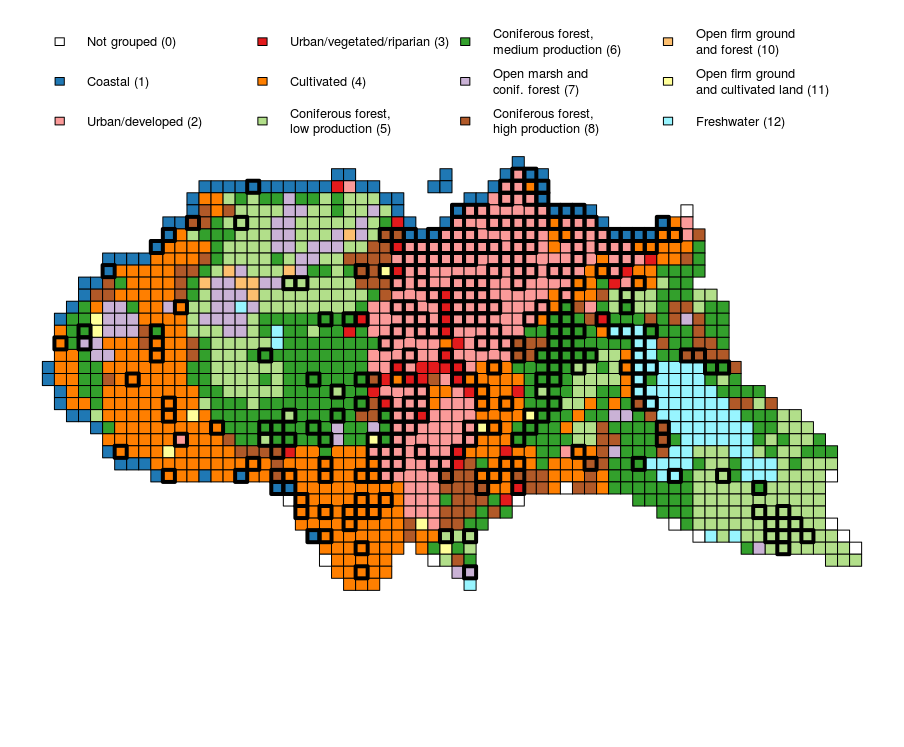
\includegraphics [width=1\textwidth]{Cluster_map_border.png}
\caption {\textbf{Trondheim Municipality coloured by habitat.} Colour definitions shown in the legend above. Grid cells used for the modelling is indicated with a black border.}
\label{fig:Clusters}\end {figure}

\begin{figure}[h]
    \centering
    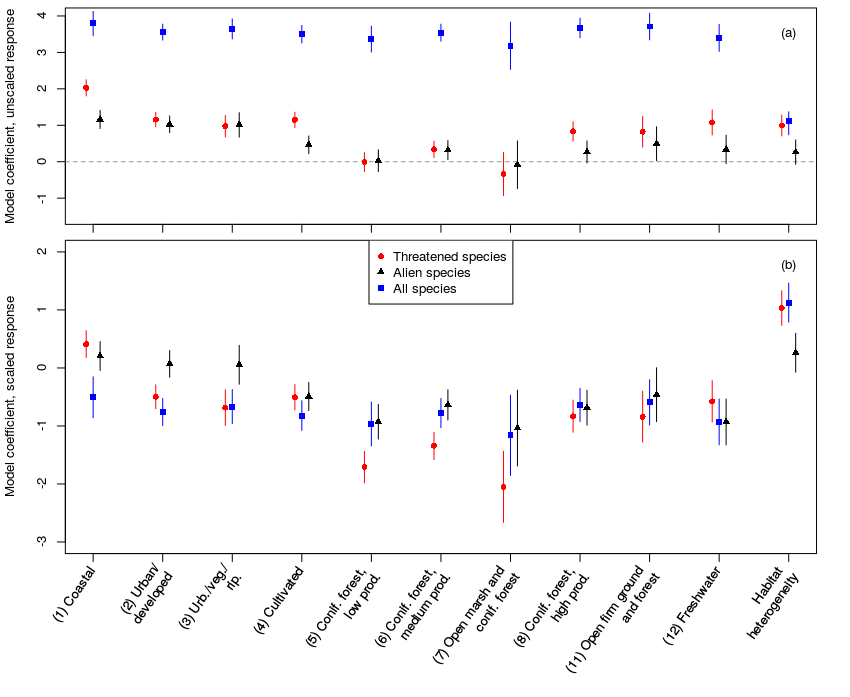
\includegraphics[width=1\textwidth]{coef.png}
    \caption{\textbf{Model coefficients for the models of ESR.} \textbf{(a)} Model coefficients for the unscaled response variable, showing the numerical differences in species richness between the models, and \textbf{(b)} model coefficients for the scaled response variable, showing the relative difference in effect size between the models. Figures denote the coefficient value, lines show the Standard Error of the estimate.\\
    Each coefficient (incl. standard errors) corresponds to the coefficient value when the model is re-fitted with the corresponding factor level as intercept. For the threatened species, the standard errors are as returned by the models, for the averaged models (all species and alien species), the adjusted standard errors are depicted. }
    \label{fig:coefficients}
\end{figure}

\begin{figure}
    \centering
    \subfloat[]{
        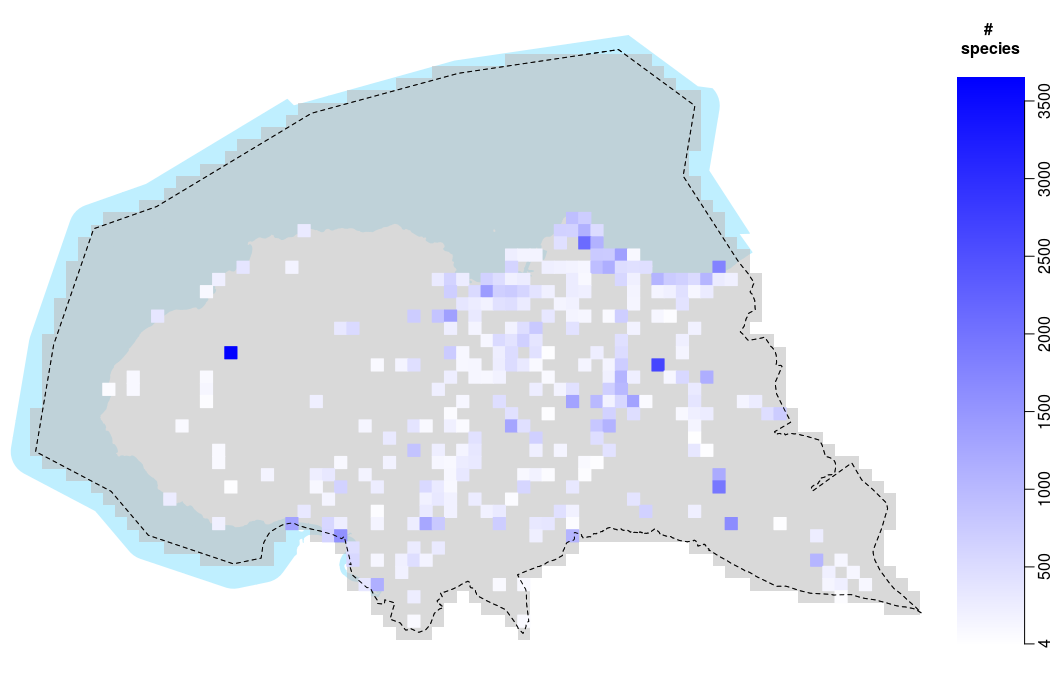
\includegraphics[width=0.48\textwidth]{ESR_all.png}
        \label{fig:ESR_all}   }
        \hfill
    \subfloat[]{
        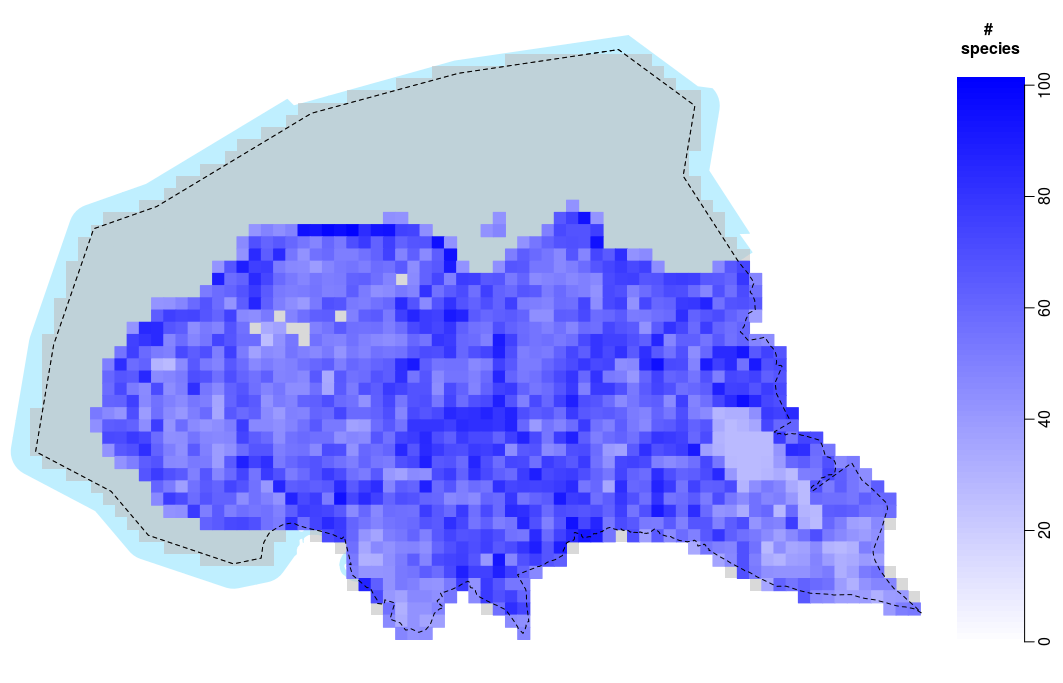
\includegraphics[width=0.48\textwidth]{predict_all.png}
        \label{fig:predict_all}     }
        
    \subfloat[]{
        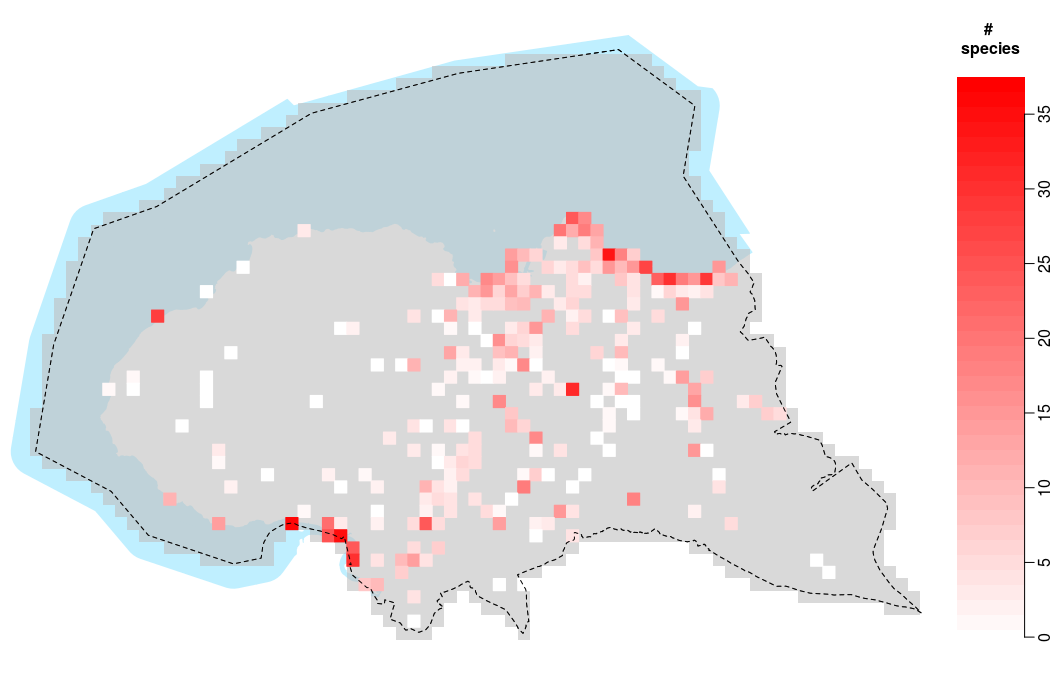
\includegraphics[width=0.48\textwidth]{ESR_threatened.png}
        \label{fig:ESR_threatened}  }
        \hfill
    \subfloat[]{
        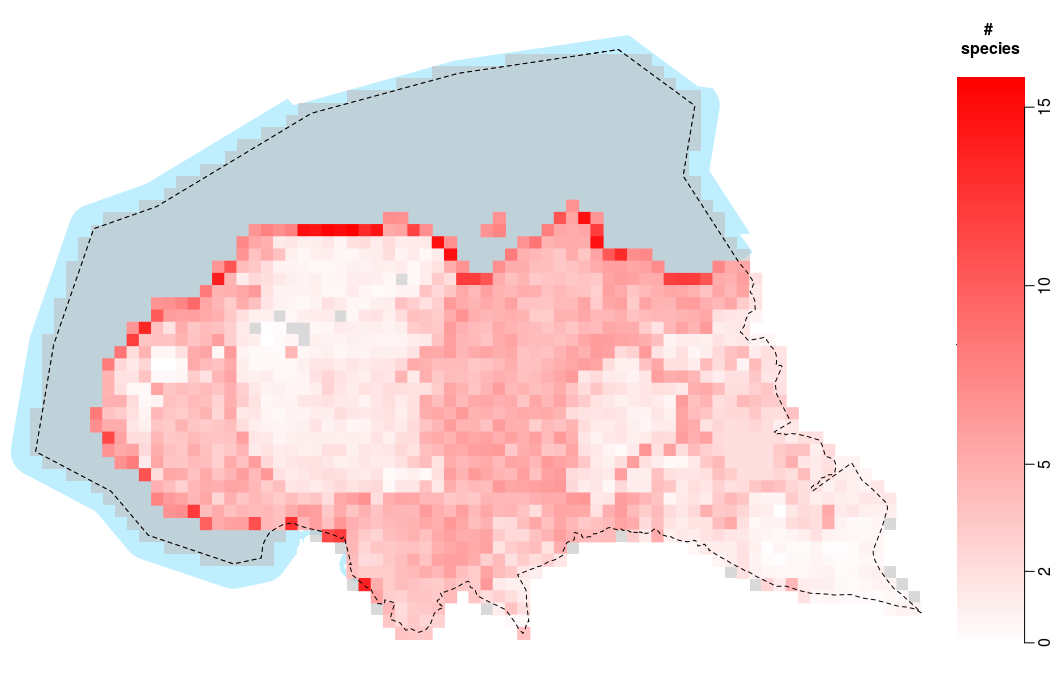
\includegraphics[width=0.48\textwidth]{predict_threatened.png}
        \label{fig:predict_threatened}  }
        
    \subfloat[]{
        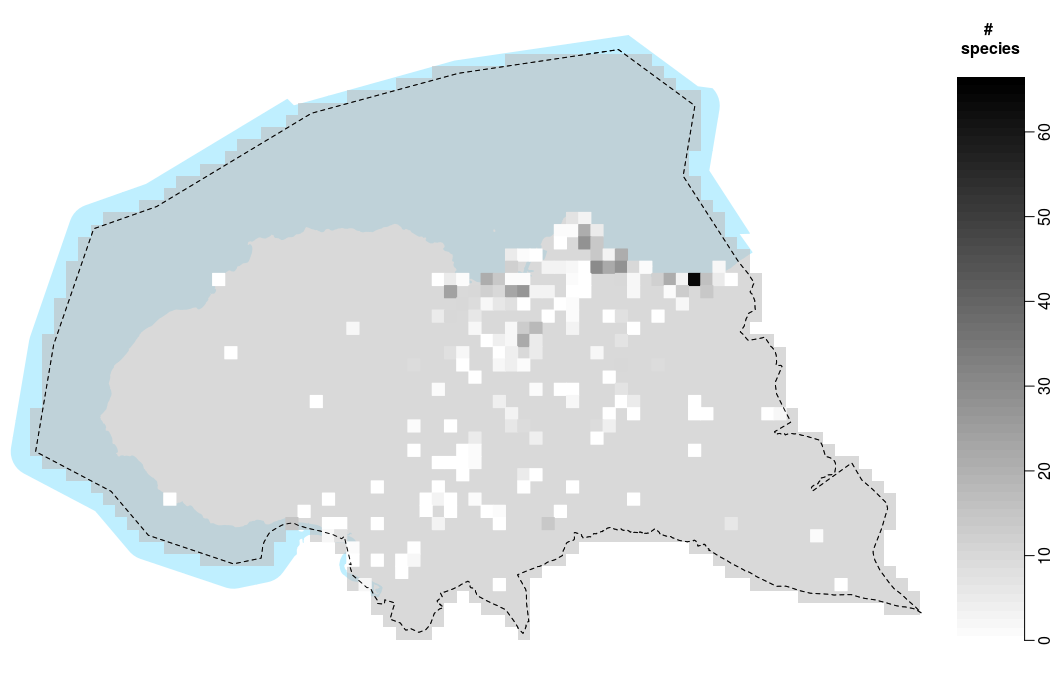
\includegraphics[width=0.48\textwidth]{ESR_alien.png}
        \label{fig:ESR_alien}   }
        \hfill
    \subfloat[]{
        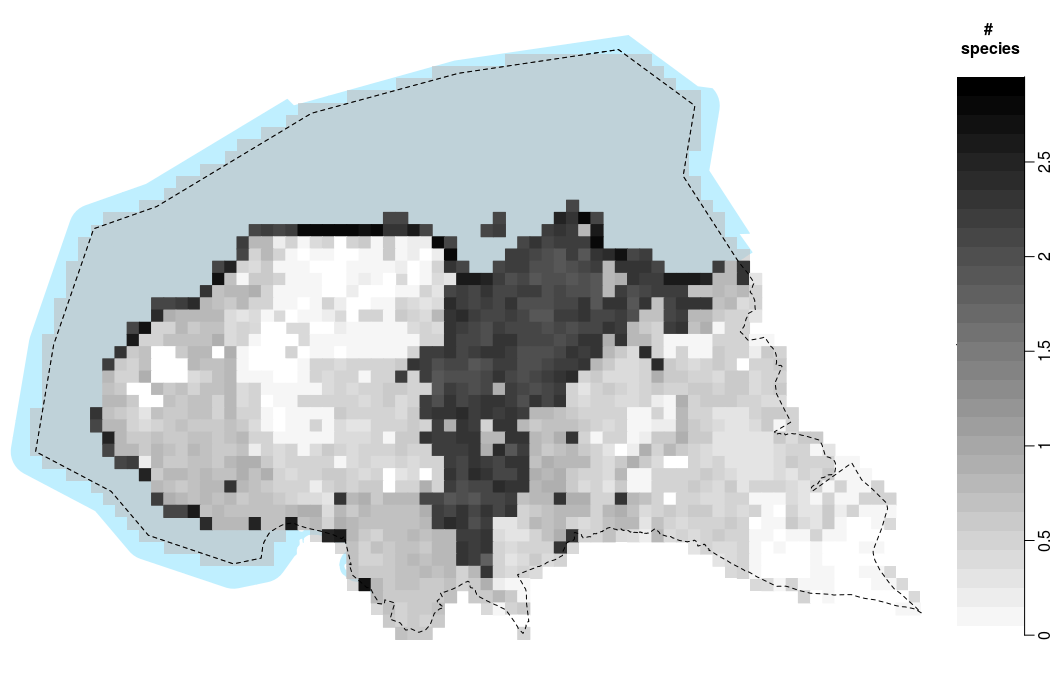
\includegraphics[width=0.48\textwidth]{predict_alien.png}
        \label{fig:predict_alien}}
    \caption{\textbf{Extrapolated Species Richness used for model construction vs. the model predictions for Extrapolated Species Richness.} Extrapolated species richness for \textit{(a)} all species, \textit{(c)} threatened species and \textit{(e)} alien species, and model predictions of ESR for \textit{(b)} all species, \textit{(d)} threatened species and \textit{(f)} alien species. 
    The model predictions have been back-transformed from the modelled $log(x+1)$, thus the right panel shows the extrapolated number of species.}
    \label{fig:ESR_predictions}
\end{figure}

\clearpage
\section{Supplementary Material} \FloatBarrier   % Process all figures - they cannot pass this barrier
\renewcommand\thefigure{S.\arabic{figure}}
\setcounter{figure}{0}
\renewcommand\thetable{S.\arabic{table}}
\setcounter{table}{0}

\subsection{Criteria for inclusion of threatened species} \label{sec:Redlist_criteria}
\textit{Description of how the entire Red List from the Norwegian Biodiversity Information Centre was sorted. The categories from 2006, 2010 and 2015 for each species evaluated in the lists were compared:}\\

The official Norwegian Red Lists from 2006, 2010 and 2015, including the notes on the evaluations, were provided by the Norwegian Biodiversity Information Centre. The three lists provided the basis for the modified version of the Norwegian Red List used in this study. The used abbreviations are in line with the official IUCN categories:  \textit{DD} = `Data Deficient', \textit{LC} = `Least Concern', \textit{NT} = `Near Threatened', \textit{VU} = `Vulnerable', \textit{EN} = `Endangered', \textit{CR} = `Critically Endangered', \textit{RE} = `Regionally Extinct', \textit{NE} = `Not Evaluated', \textit{NA} = `Not Available'.\\
If species have not been evaluated in any year (categorized as either NA or NE), they are immediately discarded.\\
Similarly, if species have only ever been evaluated as LC, or as any combination of LC and non-evaluated, they are discarded.\\
If species have previously been evaluated to DD (on the threatened part of the Red List), but was evaluated as LC in the latest version (2015), they were discarded.\\
Species listed as LC in the previous two assessments were discarded as well, regardless of their category in 2006.\\

All species evaluated to be in the threatened categories (RE, CR, EN, VU and NT) in 2015 were included in the used Red List. Species listed as DD were evaluated separately (see the further description).\\
All species only listed within the threatened categories were included in the list (incl. combinations with NA, NE and DD - thus, species never categorised as LC).
All species evaluated as data deficient in all years (DD) were included in the final version of the Red List. Similarly, all species listed as DD once, otherwise as any combination of NE and NA, were included in the Red List.\\
All species listed as regionally extinct (RE) at any point, were included in the list.\\

For all species listed as LC, NA, NE or DD in the latest assessment (2015), but previously listed as any of the threatened categories (RE, CR, EN, VU, NT and DD), the official reasoning for down-grading of the respective species was assessed and evaluated. Generally, species where there was great uncertainty regarding the actual current status of the species, was included in the list. Otherwise, the species was discarded.\\
Description/reasoning for all of the individually evaluated species can be presented upon requests.

\newpage
\subsection{Land cover characteristic of the habitats} \label{sec:Landcover_clusters}
The characteristic AR5 land cover types of each of the habitats are evaluated based on the mean area of each land cover type within the grid cells assigned to the respective habitats. An overview of the characterising land cover types can be seen in Figure \ref{fig:spineplot}. The dominating land cover type has been determining for the used name for each of the habitats.\\
The official AR5 land cover types falling under the labels defined here are as shown in Table \ref{table:AR5_classes} (\cite{Ahlstr2014}).

\begin{figure}[!htb] 
    \centering
    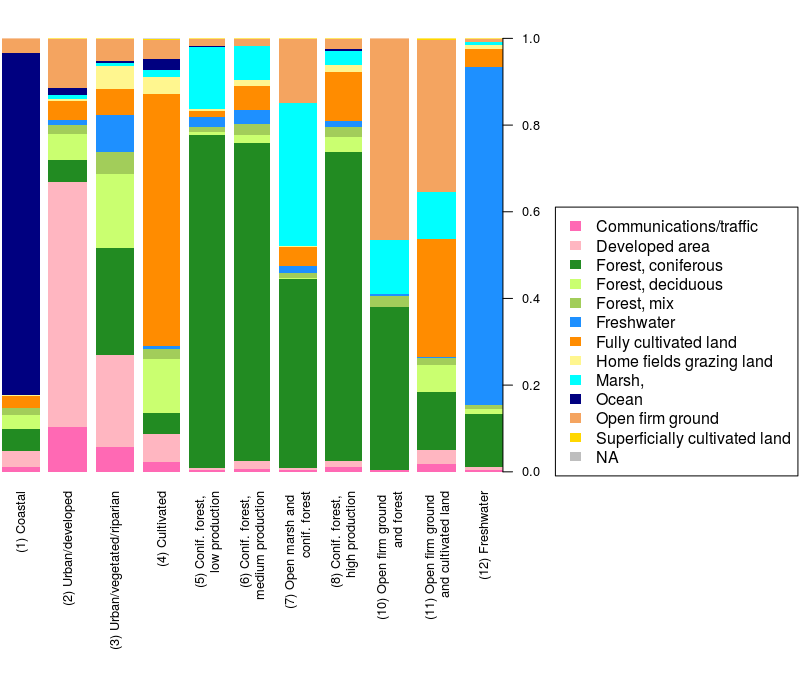
\includegraphics[width=1\textwidth]{spineplot.png}
    \caption{\textbf{Land cover within habitat categories.} Proportion of grid cell within each habitat on average covered by the respective AR5 land cover types.}
    \label{fig:spineplot}
\end{figure}


\newpage
\begin{longtable}{ p{4cm} | p{4cm} l l l} 
\caption{\textbf{Labels of AR5 land cover types in Figure \ref{fig:spineplot} and the included sub-classes.} Only sub-classes occurring within the study area are included. Categories are translated from Ahlstrøm et al. (2014).}\\
\label{table:AR5_classes}\\
\textbf{Label}          &   \textbf{Area type}      &   \textbf{Tree cover}     &       \textbf{Productivity}       &       \textbf{Soil condition} \\
\hline
Communications/traffic  &   Communications/traffic  & -                         &       -                           &       -                  \\
\hline
Developed area          & Developed area            & -                         &       -                           &       -                  \\
\hline
\multirow{15}{*}{Forest, coniferous} & \multirow{15}{*}{Forest} & \multirow{15}{*}{Coniferous} & \multirow{4}{*}{Impediment} & Bedrock \\   \cline{5-5}
                        &                           &                           &                                   &       Shallow soil \\ \cline{5-5}
                        &                           &                           &                                   &       Soil \\         \cline{5-5}
                        &                           &                           &                                   &       Organic soil \\ \cline{5-5}
\cline{4-5}
                        &                           &                           &       \multirow{4}{*}{Low}        &       Boulder \\      \cline{5-5}
                        &                           &                           &                                   &       Shallow soil \\ \cline{5-5}
                        &                           &                           &                                   &       Soil \\         \cline{5-5}
                        &                           &                           &                                   &       Organic soil \\ \cline{5-5}
\cline{4-5}
                        &                           &                           &       \multirow{3}{*}{Medium}     &       Shallow soil \\ \cline{5-5}
                        &                           &                           &                                   &       Soil \\         \cline{5-5}
                        &                           &                           &                                   &       Organic soil \\ \cline{5-5}
\cline{4-5}
                        &                           &                           &       \multirow{3}{*}{High}       &       Shallow soil \\ \cline{5-5}
                        &                           &                           &                                   &       Soil \\         \cline{5-5}
                        &                           &                           &                                   &       Organic soil \\ \cline{5-5}
\cline{4-5}
                        &                           &                           &       Very high                   &       Soil          \\ \cline{5-5}
\hline
\multirow{11}{*}{Forest, deciduous} & \multirow{11}{*}{Forest} & \multirow{11}{*}{Deciduous} &  \multirow{4}{*}{Impediment} & Bedrock \\    \cline{5-5}
                        &                           &                           &                                   &       Shallow soil \\ \cline{5-5}
                        &                           &                           &                                   &       Soil \\         \cline{5-5}
                        &                           &                           &                                   &       Organic soil \\ \cline{5-5}
\cline{4-5}
                        &                           &                           &       \multirow{2}{*}{Low}        &       Soil \\         \cline{5-5}
                        &                           &                           &                                   &       Organic soil \\ \cline{5-5}
\cline{4-5}
                        &                           &                           &       \multirow{3}{*}{Medium}     &       Shallow soil \\ \cline{5-5}
                        &                           &                           &                                   &       Soil \\         \cline{5-5}
                        &                           &                           &                                   &       Organic soil \\ \cline{5-5}
\cline{4-5}
                        &                           &                           &       \multirow{2}{*}{High}       &       Soil \\         \cline{5-5}
                        &                           &                           &                                   &       Organic soil \\ \cline{5-5}
\hline
\multirow{10}{*}{Forest, mix}   & \multirow{11}{*}{Forest} &    \multirow{11}{*}{Mix} & \multirow{3}{*}{Impediment} & Shallow soil \\       \cline{5-5}
                        &                           &                           &                                   &       Soil \\         \cline{5-5}
                        &                           &                           &                                   &       Organic soil \\ \cline{5-5}
\cline{4-5}
                        &                           &                           &       \multirow{3}{*}{Low}        &       Shallow soil \\ \cline{5-5}
                        &                           &                           &                                   &       Soil \\         \cline{5-5}
                        &                           &                           &                                   &       Organic soil \\ \cline{5-5}
\cline{4-5}
                        &                           &                           &       \multirow{3}{*}{Medium}     &       Shallow soil \\ \cline{5-5}
                        &                           &                           &                                   &       Soil \\         \cline{5-5}
                        &                           &                           &                                   &       Organic soil \\ \cline{5-5}
\cline{4-5}
                        &                           &                           &       High                        &       Soil \\         \cline{5-5}
\hline
Freshwater              &   Freshwater              &       -                   &       -                           &       -  \\       
\hline
\multirow{2}{*}{Fully cultivated land} & \multirow{2}{*}{Fully cultivated land} & \multirow{2}{*}{-}  & \multirow{2}{*}{-}  &   Soil \\     \cline{5-5}
                        &                           &                           &                                   &       Organic soil \\ \cline{5-5}
\hline
\multirow{4}{*}{Home fields grazing land} & \multirow{4}{*}{Home fields grazing land}  & Deciduous &    -           &       Soil \\         \cline{3-5}
                        &                           &   \multirow{3}{*}{-}      &    \multirow{3}{*}{-}             &       Shallow soil \\ \cline{5-5}
                        &                           &                           &                                   &       Soil \\         \cline{5-5}
                        &                           &                           &                                   &       Organic soil \\ \cline{5-5}
\hline
\multirow{9}{*}{Marsh}  & \multirow{9}{*}{Marsh}    &   Open                    &       Impediment                  &       - \\            \cline{3-5}
                        &                           & \multirow{4}{*}{Coniferous}   &   Impediment                  &       - \\            \cline{5-5}
                        &                           &                           &       Low                         &       - \\            \cline{5-5}
                        &                           &                           &       Medium                      &       - \\            \cline{5-5}
                        &                           &                           &       High                        &       - \\            \cline{3-5}
                        &                           & \multirow{2}{*}{Deciduous}    &   Impediment                  &       - \\            \cline{5-5}
                        &                           &                           &       Medium                      &       - \\            \cline{3-5}
                        &                           & \multirow{2}{*}{Mix}      &       Impediment                  &       - \\            \cline{5-5}
                        &                           &                           &       Low                         &       - \\            \cline{5-5}
\hline
Ocean                   &   Ocean                   &   -                       &       -                           &       - \\
\hline
\multirow{7}{*}{Open firm ground} & \multirow{7}{*}{Open firm ground} & \multirow{7}{*}{-} &    \multirow{5}{*}{Impediment} & Artificial surface \\ \cline{5-5}
                        &                           &                           &                                   &       Bedrock \\      \cline{5-5}
                        &                           &                           &                                   &       Boulder \\      \cline{5-5}
                        &                           &                           &                                   &       Shallow soil \\ \cline{5-5}
                        &                           &                           &                                   &       Soil \\         \cline{4-5}
                        &                           &                           &       Medium                      &       Soil \\         \cline{4-5}
                        &                           &                           &       High                        &       Soil \\
\hline
\multirow{3}{*}{\parbox{4cm}{\raggedright{Superficially cultivated land}}}
                        & \multirow{3}{*}{\parbox{4cm}{\raggedright{Superficially cultivated land}}}
                                                    & \multirow{3}{*}{-}        & \multirow{3}{*}{-}                &       Shallow Soil \\    \cline{5-5}
                        &                           &                           &                                   &       \multirow{2}{*}{Soil}   \\
                        &                           &                           &                                   &              \\
\hline
NA                      &   -                       &   -                       &       -                           &       -               \\
\hline
\end{longtable}

\clearpage
\newpage
\subsection{Model selection tables} \label{sec:model_sel}
Model selection tables for the \textit{MuMIn} \textit{``model.sel''}, all ranked by $AIC_c$. The best-ranking models with a $\Delta AIC_c < 2$ were the ones included in the model averaging. The models for species numbers are shown in Table \ref{table:model.sel} and, the models for scales ESR are shown in Table \ref{table:model.sel.std}.

\begin{table}[!ht]
    \caption{\textbf{Model selection table, unscaled ESR.} \textbf{(a)} all species, \textbf{(b)} threatened species and \textbf{(c)} alien species. Blank cells indicate that the respective variable was not included in the model, `+' indicates the inclusion of ``Habitat'' as a factorial variable. Models included in the model average are highlighted in gray.}
    \label{table:model.sel}
    \begin{tabular}{l r r r r r r r r r}
    \multicolumn{5}{c}{\textbf{\textit{(a)}  All species}} \\
    \hline
    \textbf{Model} & \textbf{Intercept} & \textbf{Habitat} & \textbf{Hab. het.} & \textbf{Northness} & \textbf{df} & \textbf{logLik} & \textbf{$AIC_c$} & \textbf{delta} & \text{weight} \\
    \hline
    \rowcolor{lightgray}
    3   &   3.582   &       &   0.997  &               &   4   &   -366.376    &   740.9   &   0.00    &   0.405   \\
    \rowcolor{lightgray}
    4   &   4.073   &   +   &   1.132  &               &   13  &   -357.063    &   741.4   &   0.55    &   0.308   \\
    7   &   3.587   &       &   0.992  &   -0.03086    &   5   &   -366.356    &   742.9   &   2.03    &   0.147   \\
    8   &   4.105   &   +   &   1.118  &   -0.10600    &   14  &   -356.806    &   743.1   &   2.24    &   0.132   \\
    1   &   4.183   &       &           &               &   3   &   -371.793    &   749.7   &   8.78    &   0.005   \\
    5   &   4.187   &       &           &   -0.07672    &   4   &   -371.670    &   751.5   &   10.59   &   0.002   \\
    2   &   4.580   &   +   &           &               &   12  &   -363.690    &   752.5   &   11.61   &   0.001   \\
    6   &   4.615   &   +   &           &   -0.13880    &   13  &   -363.266    &   753.8   &   12.95   &   0.001   \\

    \hline
    & & & & & & & & & \\
    
    \multicolumn{5}{c}{\textbf{\textit{(b)}  Threatened species}} \\
    \hline
    \textbf{Model} & \textbf{Intercept} & \textbf{Habitat} & \textbf{Hab. het.} & \textbf{Northness} & \textbf{df} & \textbf{logLik} & \textbf{$AIC_c$} & \textbf{delta} & \text{weight} \\
    \hline
    \rowcolor{lightgray}
    4   &   2.027   &   +   &   0.993  &               &   13  &   -332.646    &   692.6   &   0.00    &   0.727   \\
    8   &   2.048   &   +   &   0.985  &   -0.057150   &   14  &   -332.549    &   694.6   &   2.01    &   0.266   \\
    2   &   2.487   &   +   &           &               &   12  &   -338.762    &   702.6   &   10.04   &   0.005   \\
    6   &   2.514   &   +   &           &   -0.088770   &   13  &   -338.533    &   704.4   &   11.77   &   0.002   \\
    3   &   1.037   &       &   0.721  &               &   4   &   -356.241    &   720.6   &   28.02   &   0.000   \\
    7   &   1.036   &       &   0.722  &   0.007319    &   5   &   -356.240    &   722.7   &   30.08   &   0.000   \\
    1   &   1.473   &       &           &               &   3   &   -359.316    &   724.7   &   32.11   &   0.000   \\
    5   &   1.474   &       &           &   -0.017390   &   4   &   -359.309    &   726.8   &   34.15   &   0.000   \\

    \hline
    & & & & & & & & & \\
    
    \multicolumn{5}{c}{\textbf{\textit{(c)}  Alien species}} \\
    \hline
    \textbf{Model} & \textbf{Intercept} & \textbf{Habitat} & \textbf{Hab. het.} & \textbf{Northness} & \textbf{df} & \textbf{logLik} & \textbf{$AIC_c$} & \textbf{delta} & \text{weight} \\
    \hline
    \rowcolor{lightgray}
    4   &   1.0620  &   +   &   0.487  &               &   13  &   -357.829    &   743.0   &   0.00    &   0.396   \\
    \rowcolor{lightgray}
    2   &   1.2780  &   +   &           &               &   12  &   -359.081    &   743.3   &   0.31    &   0.339   \\
    8   &   1.0470  &   +   &   0.497  &   0.05713     &   14  &   -357.754    &   745.0   &   2.06    &   0.142   \\
    6   &   1.2710  &   +   &           &   0.03715     &   13  &   -359.049    &   745.4   &   2.44    &   0.117   \\
    1   &   0.7155  &       &           &               &   3   &   -373.373    &   752.8   &   9.86    &   0.003   \\
    3   &   0.5201  &       &   0.323  &               &   4   &   -372.822    &   753.8   &   10.81   &   0.002   \\
    5   &   0.7143  &       &           &   0.09253     &   4   &   -373.207    &   754.6   &   11.58   &   0.001   \\
    7   &   0.5072  &       &   0.342  &   0.10910     &   5   &   -372.593    &   755.4   &   12.42   &   0.001   \\
    \hline
    \end{tabular}
\end{table}

\begin{table}[!ht]
    \caption{\textbf{Model selection table, scaled ESR.} \textbf{(a)} all species, \textbf{(b)} threatened species and \textbf{(c)} alien species. Blank cells indicate that the respective variable was not included in the model, `+' indicates the inclusion of ``Habitat'' as a factorial variable. Models included in the model average are highlighted in gray.}
    \label{table:model.sel.std}
    \begin{tabular}{l r r r r r r r r r}
    \multicolumn{5}{c}{\textbf{\textit{(a)}  All species}} \\
    \hline
    \textbf{Model} & \textbf{Intercept} & \textbf{Habitat} & \textbf{Hab. het.} & \textbf{Northness} & \textbf{df} & \textbf{logLik} & \textbf{$AIC_c$} & \textbf{delta} & \text{weight} \\
    \hline
    \rowcolor{lightgray}
    3   &   -0.73330    &       &   1.064   &               &   4   &   -385.278    &   778.7   &   0.00    &   0.405   \\
    \rowcolor{lightgray}
    4   &   -0.20960    &   +   &   1.208   &               &   13  &   -375.960    &   779.2   &   0.55    &   0.308   \\
    7   &   -0.72800    &       &   1.058   &   -0.03293    &   5   &   -385.253    &   780.7   &   2.03    &   0.147   \\
    8   &   -0.17570    &   +   &   1.193   &   -0.11310    &   14  &   -375.703    &   780.9   &   2.24    &   0.132   \\
    1   &   -0.09189    &       &           &               &   3   &   -390.690    &   787.5   &   8.78    &   0.005   \\
    5   &   -0.08750    &       &           &   -0.08187    &   4   &   -390.567    &   789.3   &   10.59   &   0.002   \\
    2   &   0.33180     &   +   &           &               &   12  &   -382.587    &   790.3   &   11.61   &   0.001   \\
    6   &   0.36820     &   +   &           &   -0.14820    &   13  &   -382.163    &   791.6   &   12.95   &   0.001   \\

    \hline
    & & & & & & & & & \\
    
    \multicolumn{5}{c}{\textbf{\textit{(b)}  Threatened species}} \\
    \hline
    \textbf{Model} & \textbf{Intercept} & \textbf{Habitat} & \textbf{Hab. het.} & \textbf{Northness} & \textbf{df} & \textbf{logLik} & \textbf{$AIC_c$} & \textbf{delta} & \text{weight} \\
    \hline
    \rowcolor{lightgray}
    4   &   0.4095   &   +   &   1.033  &               &   13  &   -344.006    &   715.3   &   0.00    &   0.727   \\
    8   &   0.4313   &   +   &   1.024  &   -0.05942    &   14  &   -343.908    &   717.3   &   2.01    &   0.266   \\
    2   &   0.8872   &   +   &           &               &   12  &   -350.121    &   725.4   &   10.04   &   0.005   \\
    6   &   0.9158   &   +   &           &   -0.09231    &   13  &   -349.892    &   727.1   &   11.77   &   0.002   \\
    3   &   -0.6203  &       &   0.749  &               &   4   &   -367.601    &   743.3   &   28.02   &   0.000   \\
    7   &   -0.6212  &       &   0.750  &   0.00761     &   5   &   -367.600    &   745.4   &   30.08   &   0.000   \\
    1   &   -0.1664  &       &           &               &   3   &   -370.675    &   747.4   &   32.11   &   0.000   \\
    5   &   -0.1656  &       &           &   -0.01808    &   4   &   -370.669    &   749.5   &   34.15   &   0.000   \\

    \hline
    & & & & & & & & & \\
    
    \multicolumn{5}{c}{\textbf{\textit{(c)}  Alien species}} \\
    \hline
    \textbf{Model} & \textbf{Intercept} & \textbf{Habitat} & \textbf{Hab. het.} & \textbf{Northness} & \textbf{df} & \textbf{logLik} & \textbf{$AIC_c$} & \textbf{delta} & \text{weight} \\
    \hline
    \rowcolor{lightgray}
    4   &   0.10550  &   +   &   0.486  &               &   13  &   -357.101    &   741.5   &   0.00    &   0.396   \\
    \rowcolor{lightgray}
    2   &   0.32100  &   +   &           &               &   12  &   -358.352    &   741.8   &   0.31    &   0.339   \\
    8   &   0.09003  &   +   &   0.496  &   0.05699     &   14  &   -357.025    &   743.6   &   2.06    &   0.142   \\
    6   &   0.31370  &   +   &           &   0.03706     &   13  &   -358.320    &   744.0   &   2.44    &   0.117   \\
    1   &   -0.24030 &       &           &               &   3   &   -372.644    &   751.4   &   9.86    &   0.003   \\
    3   &   -0.43530 &       &   0.322  &               &   4   &   -372.093    &   752.3   &   10.81   &   0.002   \\
    5   &   -0.24150 &       &           &   0.09230     &   4   &   -372.478    &   753.1   &   11.58   &   0.001   \\
    7   &   -0.44810 &       &   0.341  &   0.10880     &   5   &   -371.864    &   753.9   &   12.42   &   0.001   \\
    \hline
    \end{tabular}
\end{table}

\newpage

\subsection{Averaged models} \label{sec:models}
\begin{table}[h]  % Figure out what the y-axis actually means - so some more specific interpretations of the values
    \caption{\textbf{Averaged Generalized Least Squared models.} (Unscaled) Extrapolated Species Richness for \textbf{(a)} all species, \textbf{(b)} threatened species and \textbf{(c)} alien species. "Urban/developed" is used as the intercept, and the categorical habitats are thus relative to this. As only one model was deemed ``best'' for the threatened species, no average model was constructed, and the highest ranking model is reported.}
    \label{table:model_parameters}
    \begin{tabular}{l r r r r r}
    \multicolumn{3}{c}{\textbf{\textit{(a)}  All species}} & \multicolumn{3}{c}{$\text{Pseudo-R}^2 = 0.304$} \\
    \hline
    \textbf{Variable} & \textbf{Estimate} & \textbf{Std. error} & \textbf{Adjusted SE} & \textbf{\textit{z}-value} & \textbf{\textit{p}-value} \\
    \hline
    Urban/developed                         & 3.557    & 0.218     & 0.219       & 16.246   & 0.0000    \\
    Coastal                                 & 0.237    & 0.310     & 0.310       & 0.765    & 0.4442    \\
    Urban/vegetated/riparian                & 0.089    & 0.185     & 0.186       & 0.477    & 0.6336    \\
    Cultivated                              & -0.057   & 0.134     & 0.134       & 0.428    & 0.6685    \\
    Coniferous forest, low production       & -0.193   & 0.280     & 0.281       & 0.687    & 0.4923    \\
    Coniferous forest, medium production    & -0.016   & 0.136     & 0.137       & 0.114    & 0.9095    \\
    Open marsh and coniferous forest        & -0.375   & 0.596     & 0.597       & 0.629    & 0.5295    \\
    Coniferous forest, high production      & 0.115    & 0.208     & 0.209       & 0.551    & 0.5813    \\
    Open firm ground and cultivated land    & 0.154    & 0.322     & 0.323       & 0.478    & 0.6326    \\
    Freshwater                              & -0.159   & 0.307     & 0.308       & 0.517    & 0.6050    \\
    Habitat heterogeneity                   & 1.055    & 0.314     & 0.315       & 3.352    & 0.0008    \\
    \hline
    & & & & & \\
    
    \multicolumn{3}{c}{\textbf{\textit{(b)}  Threatened species}} & \multicolumn{3}{c}{$\text{Pseudo-R}^2 = 0.594$} \\
    \hline
    \textbf{Variable} & \textbf{Estimate} & \textbf{Std. error} & \textbf{Adjusted SE} & \textbf{\textit{t}-value} & \textbf{\textit{p}-value} \\
    \hline
    Urban/developed                         & 1.155    & 0.198     & -       & 5.838    & 0.0000    \\
    Coastal                                 & 0.872    & 0.201     & -       & 4.342    & 0.0000    \\
    Urban/vegetated/riparian                & -0.179   & 0.218     & -       & -0.823   & 0.4111    \\
    Cultivated                              & -0.008   & 0.153     & -       & -0.050   & 0.9605    \\
    Coniferous forest, low production       & -1.165   & 0.222     & -       & -5.259   & 0.0000    \\
    Coniferous forest, medium production    & -0.814   & 0.173     & -       & -4.704   & 0.0000    \\
    Open marsh and coniferous forest        & -1.493   & 0.565     & -       & -2.642   & 0.0087    \\
    Coniferous forest, high production      & -0.321   & 0.217     & -       & -1.482   & 0.1396    \\
    Open firm ground and cultivated land    & -0.331   & 0.386     & -       & -0.858   & 0.3917    \\
    Freshwater                              & -0.076   & 0.317     & -       & -0.241   & 0.8095    \\
    Habitat heterogeneity                   & 0.993    & 0.286     & -       & 3.468    & 0.0006    \\
    \hline
    & & & & & \\
    
    \multicolumn{3}{c}{\textbf{\textit{(c)}  Alien species}} & \multicolumn{3}{c}{$\text{Pseudo-R}^2 = 0.473$} \\
    \hline
    \textbf{Variable} & \textbf{Estimate} & \textbf{Std. error} & \textbf{Adjusted SE} & \textbf{\textit{z}-value} & \textbf{\textit{p}-value} \\
    \hline
    Urban/developed                         & 1.027    & 0.230     & 0.230       & 4.459    & 0.0000    \\
    Coastal                                 & 0.135    & 0.222     & 0.223       & 0.606    & 0.5446    \\
    Urban/vegetated/riparian                & -0.016   & 0.239     & 0.240       & 0.067    & 0.9468    \\
    Cultivated                              & -0.563   & 0.170     & 0.171       & 3.296    & 0.0010    \\
    Coniferous forest, low production       & -1.000   & 0.248     & 0.249       & 4.018    & 0.0001    \\
    Coniferous forest, medium production    & -0.708   & 0.194     & 0.195       & 3.636    & 0.0003    \\
    Open marsh and coniferous forest        & -1.110   & 0.620     & 0.623       & 1.783    & 0.0745    \\
    Coniferous forest, high production      & -0.757   & 0.240     & 0.241       & 3.144    & 0.0017    \\
    Open firm ground and cultivated land    & -0.533   & 0.419     & 0.420       & 1.269    & 0.2046    \\
    Freshwater                              & -0.689   & 0.355     & 0.357       & 1.933    & 0.0532    \\
    Habitat heterogeneity                   & 0.263    & 0.334     & 0.335       & 0.784    & 0.4333    \\
    \hline
    \end{tabular}
\end{table}

\FloatBarrier
\begin{figure}[!h]
    \centering
    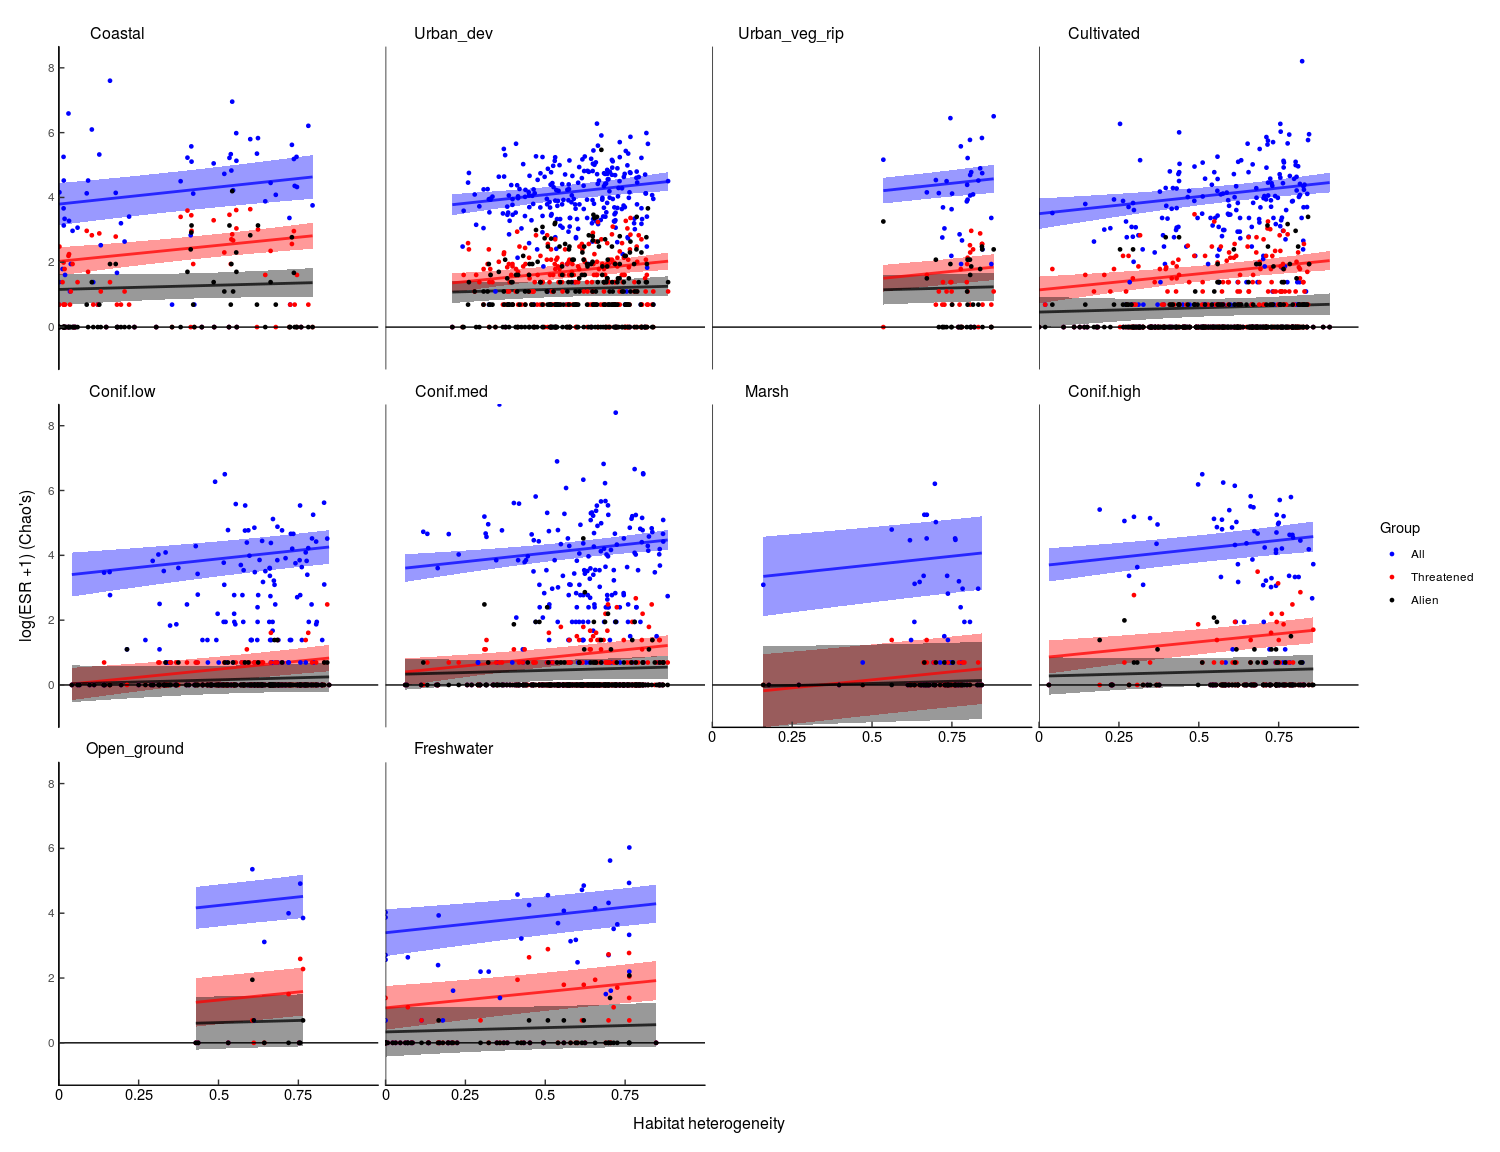
\includegraphics[width=1\textwidth]{Predictions_ribbon.png}
    \caption{\textbf{Model predictions (unscaled ESR).} Lines indicate model predictions, coloured ribbons indicate standard errors. Points indicate observed values. Both models and observations are separated by habitat.}
    \label{fig:pred_ribbon}
\end{figure}

\FloatBarrier
\begin{table}[h]
    \caption{\textbf{Averaged Generalized Least Squared models.} (Scaled) Extrapolated Species Richness for \textbf{(a)} all species, \textbf{(b)} threatened species and \textbf{(c)} alien species. "Urban/developed" is used as the intercept, and the categorical habitats are thus relative to this. As only one model was deemed ``best'' for the threatened species, no average model was constructed, and the highest ranking model is reported.}
    \label{table:model_parameters.std}
    \begin{tabular}{l r r r r r}
    \multicolumn{3}{c}{\textbf{\textit{(a)}  All species}} & \multicolumn{3}{c}{$\text{Pseudo-R}^2 = 0.304$} \\
    \hline
    \textbf{Variable} & \textbf{Estimate} & \textbf{Std. error} & \textbf{Adjusted SE} & \textbf{\textit{z}-value} & \textbf{\textit{p}-value} \\
    \hline
    Urban/developed                         & -0.760   & 0.233     & 0.234       & 3.255    & 0.0011    \\
    Coastal                                 & 0.253    & 0.331     & 0.331       & 0.765    & 0.4442    \\
    Urban/vegetated/riparian                & 0.095    & 0.198     & 0.199       & 0.477    & 0.6336    \\
    Cultivated                              & -0.061   & 0.143     & 0.143       & 0.428    & 0.6685    \\
    Coniferous forest, low production       & -0.206   & 0.299     & 0.300       & 0.687    & 0.4923    \\
    Coniferous forest, medium production    & -0.017   & 0.145     & 0.146       & 0.114    & 0.9095    \\
    Open marsh and coniferous forest        & -0.400   & 0.636     & 0.637       & 0.629    & 0.5295    \\
    Coniferous forest, high production      & 0.123    & 0.222     & 0.223       & 0.551    & 0.5813    \\
    Open firm ground and cultivated land    & 0.165    & 0.344     & 0.345       & 0.478    & 0.6326    \\
    Freshwater                              & -0.170   & 0.328     & 0.329       & 0.517    & 0.6050    \\
    Habitat heterogeneity                   & 1.126    & 0.335     & 0.336       & 3.352    & 0.0008    \\
    \hline
    & & & & & \\
    
    \multicolumn{3}{c}{\textbf{\textit{(b)}  Threatened species}} & \multicolumn{3}{c}{$\text{Pseudo-R}^2 = 0.594$} \\
    \hline
    \textbf{Variable} & \textbf{Estimate} & \textbf{Std. error} & \textbf{Adjusted SE} & \textbf{\textit{t}-value} & \textbf{\textit{p}-value} \\
    \hline
    Urban/developed                         & -0.497   & 0.206     & -       & -2.417    & 0.0163    \\
    Coastal                                 & 0.907    & 0.209     & -       & 4.342    & 0.0000    \\
    Urban/vegetated/riparian                & -0.187   & 0.227     & -       & -0.823   & 0.4111    \\
    Cultivated                              & -0.008   & 0.159     & -       & -0.050   & 0.9605    \\
    Coniferous forest, low production       & -1.212   & 0.230     & -       & -5.259   & 0.0000    \\
    Coniferous forest, medium production    & -0.847   & 0.180     & -       & -4.704   & 0.0000    \\
    Open marsh and coniferous forest        & -1.552   & 0.588     & -       & -2.642   & 0.0087    \\
    Coniferous forest, high production      & -0.334   & 0.226     & -       & -1.482   & 0.1396    \\
    Open firm ground and cultivated land    & -0.344   & 0.401     & -       & -0.858   & 0.3917    \\
    Freshwater                              & -0.080   & 0.330     & -       & -0.241   & 0.8095    \\
    Habitat heterogeneity                   & 1.033    & 0.298     & -       & 3.468    & 0.0006    \\
    \hline
    & & & & & \\
    
    \multicolumn{3}{c}{\textbf{\textit{(c)}  Alien species}} & \multicolumn{3}{c}{$\text{Pseudo-R}^2 = 0.473$} \\
    \hline
    \textbf{Variable} & \textbf{Estimate} & \textbf{Std. error} & \textbf{Adjusted SE} & \textbf{\textit{z}-value} & \textbf{\textit{p}-value} \\
    \hline
    Urban/developed                         & 0.070    & 0.230     & 0.230       & 0.305    & 0.7606    \\
    Coastal                                 & 0.135    & 0.222     & 0.223       & 0.606    & 0.5446    \\
    Urban/vegetated/riparian                & -0.016   & 0.239     & 0.239       & 0.067    & 0.9468    \\
    Cultivated                              & -0.562   & 0.170     & 0.170       & 3.296    & 0.0010    \\
    Coniferous forest, low production       & -0.998   & 0.247     & 0.248       & 4.018    & 0.0001    \\
    Coniferous forest, medium production    & -0.707   & 0.194     & 0.194       & 3.636    & 0.0003    \\
    Open marsh and coniferous forest        & -1.108   & 0.619     & 0.621       & 1.783    & 0.0745    \\
    Coniferous forest, high production      & -0.755   & 0.239     & 0.240       & 3.144    & 0.0017    \\
    Open firm ground and cultivated land    & -0.532   & 0.417     & 0.419       & 1.269    & 0.2046    \\
    Freshwater                              & -0.688   & 0.354     & 0.356       & 1.933    & 0.0532    \\
    Habitat heterogeneity                   & 0.262    & 0.334     & 0.334       & 0.784    & 0.4333    \\
    \hline
    \end{tabular}
\end{table}
%%C:endignore

\end{document}